\section{Análisis de la obra escultórica: Cristo de la Síndone de Miñarro} 

%\begin{figure}[ht!]
%    \centering
%    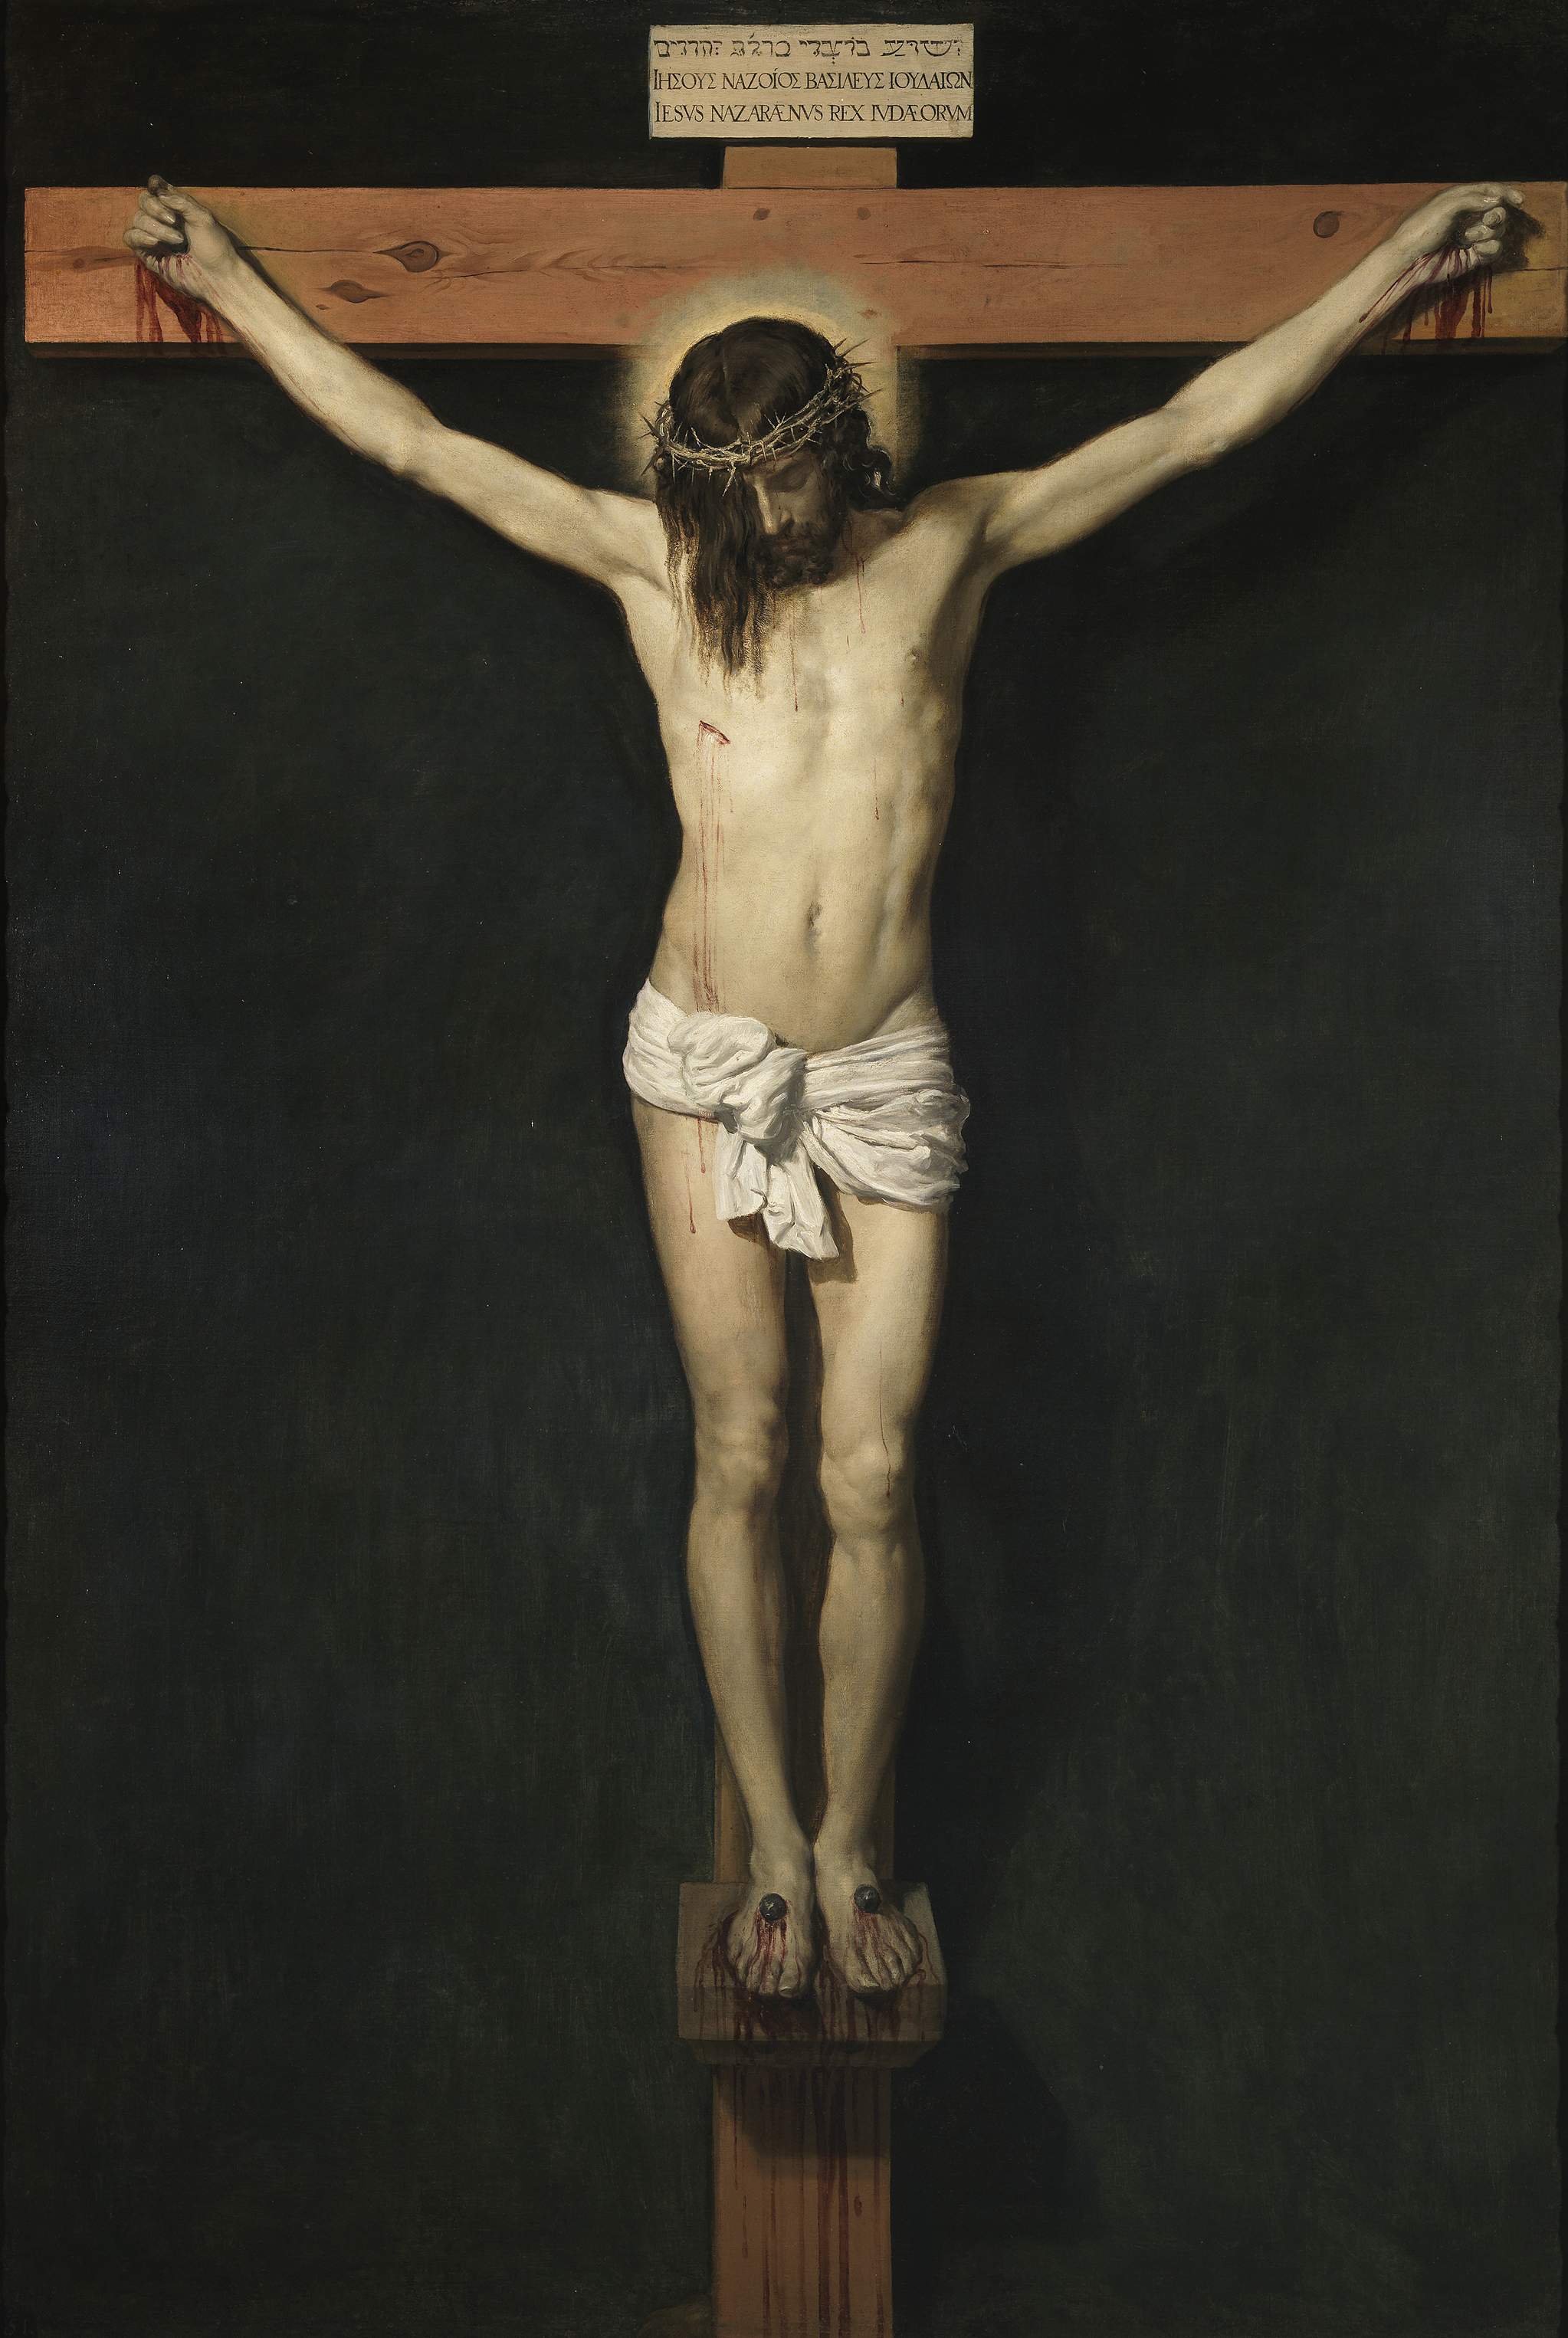
\includegraphics[width=1.0\textwidth]{velazquez.jpg}
%   .\caption{Cristo crucificado de Velázquez. Museo nacional del Prado} %. URL: www.museodelprado.es/coleccion/galeria-on-line/galeria-on-line/zoom/1/obra/cristo-crucificado-1/oimg/0/}
%\end{figure}

\newpage

%Arte, estilo: Barroco
%Cronología: 1632
%Lugar: Museo del Prado, Madrid, España
%Autor: Diego Velázquez
%Título: Cristo crucificado

%Función: Aunque se encontraba en el Convento de la encarnación de San Plácido, no está claro donde estuvo los primeros años tras su realización ni la función específica que desarrollaba. Posteriormente se tiene constancia de que estuvo en la sacristía de este convento hasta alrededor del 1804, año en el que Godoy lo compra al convento. Pasa después por distintas manos, llegando finalmente al Museo de Prado en 1829, donde permanece actualmente.
% El Cristo crucificado de velazquez, trasfondo histórico religioso. 
% http://www.museodelprado.es/coleccion/galeria-on-line/galeria-on-line/obra/cristo-crucificado-1/

\begin{description}
\item[Estilo] Actual
\item[Cronología] 2009-2010
\item[Lugar] 
\item[Autor] Juan Manuel Miñarro
\item[Título] Cristo de la Síndone o Sindónico
\end{description}

\textbf{Contexto histórico:} Esta obra es finalizada en 2010, tras más de nueve años empleados por el autor en su elaboración. El autor pretende mostrar lo más fielmente posible la realidad de la muerte de Cristo. Se basa, por tanto, en una de las reliquias más conocidas, junto con el sudario de Oviedo, que posee relación con la muerte de Cristo: la Síndone de Turín o Sábana Santa, realizando mediante el estudio meticuloso de ésta una impresionante escultura.

Aunque no está demostrado científicamente que la Síndone fuese la sábana que envolvió a Cristo tras su muerte, presenta ciertas características que han hecho que los expertos y estudiosos de todo el mundo la identifiquen como tal. Una característica que contribuye a ello es la propia imagen que conserva grabada, que por un lado posee las características propias de un hombre torturado y crucificado de la misma forma que Cristo según los evangelios, y que por otro lado se considera imposible de falsificar con las técnicas de las que se disponen hoy en día y más difícilmente aún en cualquier época anterior, puesto que es algo no se puede crear ni de forma natural ni de forma artificial.

En su búsqueda de la realidad el autor refleja de forma impecable las heridas, contusiones, laceraciones y demás aspectos que proveen a la obra de un dramatismo nunca visto hasta ahora en la muerte de Cristo ni en obras pictóricas ni escultóricas. Además plasma todos aquellos detalles que identifican a Cristo como un hombre torturado a la hora de su muerte.

\vspace{12pt}
\textbf{Anatomía de superficie:}

En esta obra se nos muestra a un Cristo muy estudiado desde absolutamente todas y cada un de las perspectivas desde las que se puede tener en cuenta: en su anatomía, en la reproducción de la muerte y en la representación de las heridas y contusines.

Al centrarnos en el primer punto se puede ver

En esta obra Velázquez nos cautiva con una figura con una postura serena y de proporciones y anatomía estudiadas.  Responde a un modelo de siete cabezas y media. Su longitud con los brazos extendidos es igual a su altura y el ángulo que forman entre ellos es de 115º.

El autor, no se centra demasiado en la reproducción de la muerte de la figura. De hecho, aunque la cabeza de la figura caiga sobre su pecho, pudiendo sugerir la muerte de éste, tal y como apreciamos la músculatura de la espalda, brazos y piernas da la impresión de que todavía se encuentra con vida. Se podría pensar que en lugar de haber fallecido, el Cristo representado se encuentra en una posición de descanso tras el sufrimiento experimentado antes de la crucifixión. Los brazos se encuentran extendidos ambos lados del cuerpo y los músculos del brazo y de la espalda que contribuyen a ello están claramente contraídos y extendidos, contrariamente a lo que ocurriría si Cristo ya hubiese perecido, en cuyo caso la musculatura permanecería laxa y exánime.

Por la posición de las piernas, donde podemos apreciar que, al tener ambos pies apoyados, carga el peso sobre el lado izquierdo, flexionando la articulación de la rodilla de este lado e iclinando la cadera hacia el lado contrario ligeramente, es también evidente que Cristo no ha fallecido aún. El autor utiliza este ligerísimo contrapposto clásico como elemento embellecedor de la obra dejando de lado la indudable incapacidad de una persona crucificada y fallecida o al borde del fallecimiento para realizar esta acción.

Además, la figura no muestra la lividez típica de un cadáver, todo lo contrario, la figura posee el color de una persona totalmente sana, a pesar de la pérdida de sangre que Cristo debió experimentar durante su calvario. Otro detalle importante de la obra es la escasa sangre que emana de las heridas de Cristo: apenas varias gotas en las heridas de los clavos y aún menos en la herida de lanza que muestra en el costado derecho. Un rasgo de la obra que  manifiesta la muerte de Cristo, que como ya he dicho para nada está representada, es precisamente esta herida del costado, la cual en teoría fue realizada postmortem, como verificación de la muerte.

Una serie de músculos colaboran en la consecución de la postura en la que se encuentra la figura a analizar.

La espalda se encuentra erguida, los músculos que se encargan de mantener esta postura son los principales erectores de la columna: los músculos del grupo iliocostal, los del grupo longuísimo y los del espinoso.

El músculo dorsal ancho, que además se puede apreciar en la obra, proviene de la espalda e inserta en el ángulo inferior de la escápula. Su tendón estrecho envuelve al músculo redondo mayor que forma el pliegue posterior de la axila. Ambos músculos junto con el pectoral mayor, el que además forma el pliegue anterior de la axila, elevan el tronco cuando los brazos se encuentran fijos, como es el caso de la figura examinada.

El músculo trapecio, cuya principal función es la elevación de la escápula, también se observa. El serrato anterior gira la escápula y, por tanto, junto con el músculo trapecio y el elevador de la escápula que la elevan hacen que la cavidad glenoidea se oriente hacia arriba y adelante, como en la figura de la obra de Velázquez.
El deltoides, que se ve fácilmente redondeando y sustentando la articulación del hombro por su parte superior, es el principal abductor del brazo, ya que sigue el movimiento abductor que el músculo supraespinoso inicia, por lo que tiene gran relevancia en la posición de crucifixión en la que ambos brazos se encuentran en posición de abducción.

En el brazo se observan tanto el bíceps como el tríceps. El bíceps forma una prominencia en la parte anterior del brazo y se encarga de la supinación del antebrazo, la cual realiza con la ayuda del músculo supinador. El tríceps por su parte se encarga de la extensión de la articulación del codo. En este movimiento le secunda el músculo ancóneo, que no es visible en la figura de la obra analizada por encontrarse en la parte posterior del codo.

La mano se encuentra en posición de reposo en la que las articulaciones falángicas y metacarpofalángicas se encuentran ligeramente flexionadas. El músculo palmar largo contribuye sutilmente a la flexión de las articulaciones metacarpofalángicas, que es realizada fundamentalmente por los músculos flexores de los dedos.

Al tratarse de un individuo delgado y favorecido por la postura en que se encuentra (brazos estirados hacia los lados y hacia arriba) se puede intuir la caja torácico perfectamente. El borde costal inferior formado por las seis últimas costillas es fácilmente visible, al igual que la depresión en la que se encuentra el cuerpo del esternón y el contorno de algunas costillas (probablemente la cuarta, quinta, sexta y séptima).

En el abdomen se encuentran los músculos abdominales, que se pueden apreciar, aunque no muy marcados. Estos músculos forman una vaina fibrosa a cada lado de la línea media. Ambas vainas se unen en esta, formando la línea alba. También se divisa bastante bien la línea semilunar, que marca el borde lateral del músculo recto del abdomen cuya principal función en la figura es el mantenimiento de la postura erecta apoyando así a los músculos erectores de la columna.

El músculo mas superficial de los músculos laminares del abdomen es el oblicuo externo. Este entre la espina y la tuberosidad púbica gira sobre sí mismo y forma el ligamento inguinal. La depresión que suele haber a la altura de ese ligamento, y que suele ser más visible en hombre, se puede observar perfectamente en la obra pictórica.

La posición de las piernas, en las que la rodilla derecha de la figura se encuentran una en posición de extensión, mientras que la otra se encuentra ligeramente flexionada, colaboran varios músculos. Los encargados de la extensión son: el cuadriceps y los músculos del tracto iliotibial, y los de la flexión son: los músculos poplíteos y los gemelos. Al estar de pie soportando el peso sobre una pierna, el lado de la pelvis que no soporta el peso se eleva. Esta acción está realizada por los glúteos medio y menor y deja a la vista la espina ilíaca del lado derecho.
La rótula o patella se puede apreciar, al igual que la tuberosidad tibial, sobre todo en la rodilla flexionada.

Los pies se encuentran apoyados en una tabla, soportando el peso del cuerpo, y se ubican en paralelo entre ellos ligeramente separados anteriormente, con un clavo en cada dorso y sangre que emana de la herida. En la parte anterior de éstos, los dedos se encuentran relajados..